\section{Literature Summaries}
% TODO: add general explanation for the art gallery problem
This section offers an overview of previous works addressing the Art Gallery Problem \cite{o1987art}. The Art Gallery Problem \cite{o1987art} can be introduced as: given a simple planar polygon $\mathcal P$, we are interested in finding the minimum number of guards (points) that are able to see the whole polygon. A simple planar polygon is a polygon that does not intersect itself when drawn in a plane. and does not have holes. Thus, we can define visibility in a polygon $\mathcal P \subset \mathbb R^2$ as a point (guard) $p \in \mathcal P$ being able to see another point $q \in \mathcal P$ if the line segment $\overline{pq} \subseteq \mathcal P$. The points that are visible from $p$ form the visibility polygon (region) $\mathcal V(p)$. The guards that see the whole polygon $\mathcal P$ form the resulting guard set $S$.

Figure \ref{fig:art} displays an example of The Art Gallery Problem \cite{o1987art} with polygon $\mathcal P$ guarded by 4 points forming the guard set $S$. The visibility region $\mathcal V$ of each guard is marked with a different colour. For point $p \in S$, its visibility region $\mathcal V(p)$ is emphasised with the pink contour. In this case, the vertex $r$ blocks part of the view of $p$ and is called ``reflex'', because the angle it forms on the inside of the polygon is larger than $180^\circ$. Because reflex vertices are only found in concave polygons, convex polygons can then be guarded by only one guard.

\begin{figure}[h!]
    \centering
    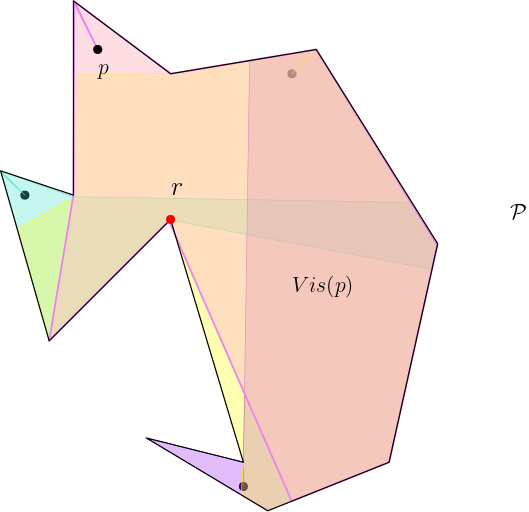
\includegraphics[width = 0.6\textwidth]{p.png}
    \caption{The Art Gallery Problem \cite{o1987art} Example}
    \label{fig:art}
\end{figure}
Building on the aforementioned concepts, the papers summarised will inspect how visibility in polygons can be efficiently computed \cite{DBLP:journals/corr/BungiuHHHK14}, how it is not always possible to place guards at rational coordinates \cite{abrahamsen2021art}, in addition to two improved polygon guarding algorithms \cite{maleki2022implementation}, \cite{DBLP:journals/corr/abs-2007-06920}.
% Some general notions that will appear in the papers are introduced below.

% Visibility in simple planar polygons can be defined as: given a polygon $\mathcal P \subset \mathbb R^2$, a point (guard) $p \in \mathcal P$ \textit{sees} a point $q \in \mathcal P$ if the line segment $\overline{pq} \subseteq \mathcal P$. Thus, the points that are visible from $p$ form the visibility polygon (region) $\mathcal V(p)$.

% A guard set $S$ is defined as a set of points in a given polygon $\mathcal P$ such that every point in $\mathcal P$ is seen by some point in $S$. $\forall x, y \in \mathcal P$, $x$ sees $y$ if the line segment $\overline{xy} \in \mathcal P$. 

\subsection{Efficient Computation of Visibility Polygons \cite{DBLP:journals/corr/BungiuHHHK14}}
This paper \cite{DBLP:journals/corr/BungiuHHHK14} introduces the implementations and their experimental evaluations for two existing algorithms (\cite{joe1987corrections}, \cite{asano1985efficient}) and a newly developed one for computing visibility in polygons. These implementations are available in the CGAL library\footnote{\url{https://www.cgal.org/}}, starting with version 4.5.

Working with the visibility region is a basic tool in computational geometry, specifically in the Art Gallery Problem \cite{o1987art}. The Art Gallery Problem \cite{o1987art} is an $\exists \mathbb R$-complete problem \cite{abrahamsen2021art}. The problem class $\exists \mathbb R$ consists of instances that can be reduced in polynomial time to a decision problem of whether a system of polynomial equations with integer coefficients and any number of real variables has a solution. Since NP $\subseteq \exists \mathbb R$, the $\exists \mathbb R$ class is an even harder to solve complexity class, since $\exists \mathbb R$ problems do not admit solutions in polynomial time. For this reason, it is crucial that the computation time of the visibility region is efficiently implemented. 

Therefore, this paper presents 3 algorithms and their implementations' performance.

\subsubsection{Algorithm of Joe and Simpson \cite{joe1987corrections}}
The algorithm of Joe and Simpson \cite{joe1987corrections} runs in $O(n)$ time and space. It begins by sequentially scanning the boundaries of the simple polygon $\mathcal P$, and adds its boundary points $v_i, \forall i = \overline{1, n}$, with $n$ the number of vertices in $\mathcal P$, to a stack $s$. For each processed edge $\overline{v_iv_{i + 1}}$, its endpoints $v_i$ and $v_{i + 1}$ are checked whether they are in the visibility region of the viewpoint $p$. If they are, $v_i$ and $v_{i + 1}$ are added to $s$. Otherwise, they are skipped. At every moment, the algorithm checks whether $\overline{v_iv_{i + 1}}$ obscures a previously added line segment. If that is the case, then the endpoints of the obscured line segment are declared obsolete and deleted. 

% The implementation of the algorithm handles the previously discussed cases for an arrangement $\mathcal P$, while also accounting for the case in which the polygon winds more than 360$^\circ$ using a winding counter.
% - **Algorithm of Joe and Simpson** $O(n)$ time and space
	% - performs a sequential scan of the boundary of $\mathcal P$ and uses a stack $s$ of boundary points $s_0, s_1, ..., s_ as summarised in the following subsections.der to deal with cases in which the polygon winds more than 360*, a winding counter is used during this edge processing
% he points that are visible from $q$ form the visibility region $\mathcal V(q)$ (polygon)

\subsubsection{Algorithm of Asano \cite{asano1985efficient}}
The algorithm of Asano \cite{asano1985efficient} runs in $O(n \log n)$ time and $O(n)$ space and uses a plane sweep approach with event line $L$. It begins by efficiently sorting all the vertices of $\mathcal P$ based on their polar angles with respect to the viewpoint $p$. For example, suppose $p$ and some given points $a_1, a_2, b_1, b_2$ are given in a plane with positive coordinates, as placed in Figure \ref{fig:asano}. The figure is taken from \cite{DBLP:journals/corr/BungiuHHHK14} and annotated in order to facilitate the explanations given in these summaries. Then, the points will be treated in the order of $b_2, b_1, a_2, a_1$ with respect to $p$ and their angular comparisons $\measuredangle b_2Oq < \measuredangle b_1Oq < \measuredangle s_1Oq < \measuredangle a_1Oq$, where $O(0, 0)$. Then, the event line $L$ starts sweeping around $p$. Every line segment that $L$ intersects is stored in a balanced binary tree $T$ in the order of intersection. As $T$ is updated, a new vertex of $\mathcal V(p)$ is stored each time the segment closest to $p$ in $T$ changes. It is important to mention that the intersection between $L$ and line segments is not explicit, but is instead determined by comparisons between the endpoints' coordinates. For instance, in Figure \ref{fig:asano}, the endpoint $b_2$ of line segment $\overline{b_2a_2}$ is the first one $L$ intersects. $b_2$ is thus added to $T$. Then, $L$ continues sweeping and adds $b_1, a_2$ and $a_1$ to $T$. Although $\overline{b_2a_2}$ and $\overline{b_1a_1}$ represent line segments $s_2$ and $s_1$, respectively, the intersection of $L$ with them is not explicitly computed, but is determined based solely on the positions of their endpoints: $s_1$ is farther away from $p$ because $q, a_2$ and $b_2$ are on the same side of $s_2$.

\begin{figure}[h!]
	\centering
	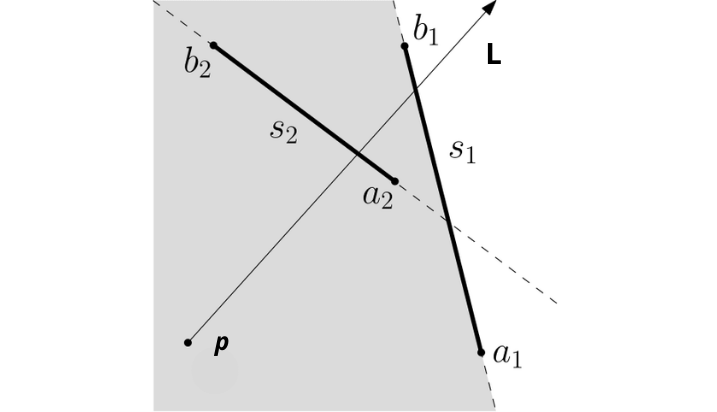
\includegraphics[width = 0.5\textwidth]{compare_segments.png}
	\caption{The Algorithm of Asano \cite{asano1985efficient} Visual Example \cite{DBLP:journals/corr/BungiuHHHK14}.}
	\label{fig:asano}
\end{figure}
	% - as the sweep proceeds, $T$ is updated and a neq vertex of $V(q)$ is generated each time the smallest element (segment closest to $q$) in $T$ changes
	% - important to have efficient comparison ops (e.g.: *add pic*)

\subsubsection{New Algorithm: Triangular Expansion}
The algorithm introduced in the paper is named Triangular Expansion and runs in $O(n^2)$ time and $O(n)$ space. It begins by triangulating $\mathcal P$ in $O(n \log n)$ time if $\mathcal P$ has holes, and $O(n)$ otherwise. Unfortunately the runtime is constrained by CGAL, which makes use of the Delaunay triangulation algorithm \cite{delaunay1934sphere} with $O(n^2)$ time for the worst case, but with better performance in practice. 

Taken from \cite{DBLP:journals/corr/BungiuHHHK14} and annotated to suit the explanations in these summaries, Figure \ref{fig:triangular} depicts an example run of the algorithm on a polygon with holes $\mathcal P$. Starting from the viewpoint $p$, the triangle containing $p$ is located by performing a simple walk. Trivially, $p$ sees the entire triangle it is contained in. The algorithm continues by recursively expanding the view of $p$ from one triangle into the other, until there are no more triangles to expand into. The view of $p$ becomes restricted by the reflex vertices $l$ and $r$ of the third triangle entered by the recursive step. Since $l$ and $r$ are reflex vertices, the view past them is further restricted until the boundaries $l'$ and $r'$ of $\mathcal P$, respectively,  are reached. Line segments $\overline{ll'}$ and $\overline{rr'}$ are added to $\mathcal V(p)$ in their angular order around $p$. At the end, $\mathcal V(p)$ will contain the segments delimiting the visibility polygon of $p$.

\begin{figure}[h!]
	\centering
	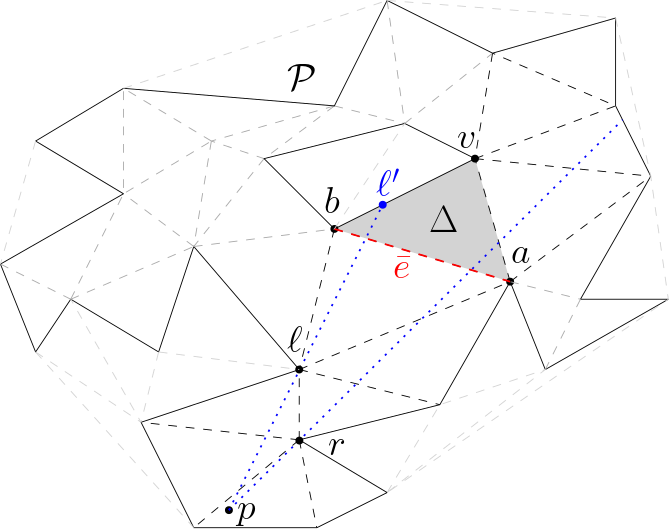
\includegraphics[width = 0.5\textwidth]{triangular_expansion.png}
	\caption{The Triangular Expansion Algorithm Example - recursion entering triangle $\Delta$ through edge $e$ \cite{DBLP:journals/corr/BungiuHHHK14}.}
	\label{fig:triangular}
\end{figure}
% - **triangular expansion** - $O(n^2)$
	% - preprocessing: triangulation ($O(n)$ for simple polygons, $O(n\log n$) for polygons with holes; Delaunay ($O(n^2)$) used)
	% - given $q$, locate the triangle containing $q$ by a simple walk ($q$ sees the entire triangle)
	% - recursive procedure that expands the view of $q$ through that edge into the next triangle. Initially, the view is restricted by the 2 endpoints of the edge, and then further as recursion continues: *add pic* for triangle $\Delta$, the view of $q$ is restricted by the 2 reflex vertices $l$ and $r$ with $a \leq r < l \leq b$ w.r.t. angular order around $q$. $v$ is a new vertex and its position w.r.t. $l$ and $r$ is computed with 2 orientation tests *add pic*: $e_l$ is a boundary edge and we can report edge $\overline{ll'}$ and $\overline{l'v}$ as part of the visibility region of $q$; $e_r$ is not a boundary edge => the recursion continues with $v$ being the vertex that now restricts the left side of the view
	% - the recursion may split into 2 calls if $e_l$ and $e_r$ are both not part of the boundary. As there are $n$ vertices, this can happen $O(n)$ times => worst-case $O(n^2)$; however a true split into two visibility cones that may reach the same triangle independently can only happen at a hole of $\mathcal P$, thus at worst the runtime is $O(nh)$, where $h$ = number of holes (linear time of simple polygons) (e.g.: worst-case *add pic*)
	% - triangulation has linear size, at most $O(n)$ recursive calls on the stack => $O(n)$ space

\subsubsection{Experiments}
The paper does not report on benchmarks with query points on edges in the interior polygon, as it claims that the implementations perform similarly to other already implemented algorithms. Instead, it uses two real-world scenarios (a simple polygon of Norway with 20981 vertices, and a cathedral polygon with 1209 vertices) and a worst-case polygon for the Triangular Expansion algorithm.

In terms of results on the real-world polygons, the Triangular Expansion algorithm has a 2-factor improved performance when compared to Asano's algorithm \cite{asano1985efficient}, and performs one order of magnitude faster than Joe and Simpson's algorithm \cite{joe1987corrections}. For the worst-case scenario, Asano's algorithm \cite{asano1985efficient} outperforms the Triangular Expansion algorithm with increasing input complexity.

Thus, despite the Triangular Expansion algorithm being outperformed in the worst-case scenario, this paper adds efficient implementations for  3 different  polygon visibility algorithms in the CGAL library. The choice of algorithms when using the library can be adapted based on the input polygons. 
% - experiments - no reports on similar benchmarks with query points on edges and in the interior polygon; for the input graphs used, the triangular expansion is 2-factor faster than Asano, and one order of magnitude faster than Joe and Simpson; with increasing input complexity, Asano does become faster
\subsection{Irrational Guards Are Sometimes Needed \cite{abrahamsen2021art}}
This paper \cite{abrahamsen2021art} studies the placement of the guards in the context of The Art Gallery Problem \cite{o1987art}. Namely, it focusses on and confirms that there are polygons with integer coordinates that require guards placed at points with irrational coordinates. Generalising, this paper shows that $\forall n \in \mathbb N$, there is a family of simple monotone polygons that can either be guarded by $3n$ guards with irrational coordinates, or $4n$ guards with rational coordinates. The result is also extended to a rectilinear polygon that can be guarded by 9 guards with irrational coordinates, or 10 guards with rational coordinates. The family of simple monotone polygons that can be guarded by $3n$ guards with irrational coordinates, as well as the rectilinear polygon that can be guarded by 9 guards with irrational coordinates are also discussed.


At the time of writing the paper, there was no combinatorial algorithm for finding an optimal solution for The Art Gallery Problem \cite{o1987art}, nor for its decidability version on whether a set $S$ of given size $k$ exists. As such, it is not known whether the problem is in NP.

First, we will address the question regarding whether polygons given by integer coordinates require guard positions with irrational coordinates in any optimal solution by introducing such a monotone polygon $\mathcal P$. A polygon is monotone if there exists a line $l$ such that every line orthogonal to $l$ intersects it at most twice. $\mathcal P$ is depicted in Figure \ref{fig:p} and is constructed using a rectangle, six triangular pockets (in green), three rectangular pockets (in blue) and four quadrilaterial pockets (in red) are added. The intuition behind the polygon will be explained in the upcoming subsections.

\begin{figure}[h!]
    \centering
    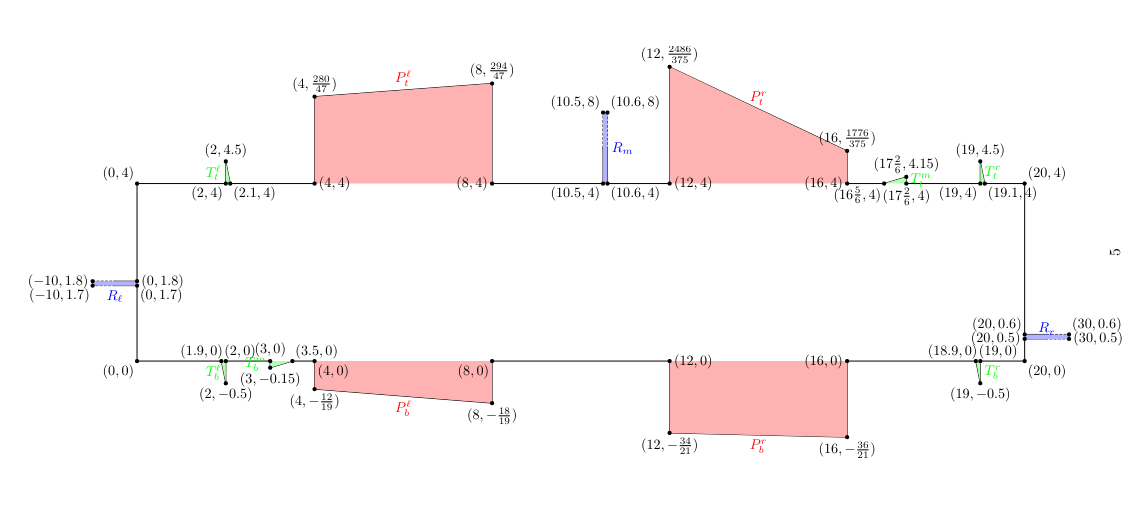
\includegraphics[width=\textwidth]{Screenshot from 2022-01-21 11-17-41.png}
    \caption{Polygon $\mathcal P$}
    \label{fig:p}
\end{figure}

\subsubsection{Intuition for Triangular Pockets}
The six triangular pockets are created in order to force a guard on a line segment. As such, they are grouped into three pairs: top pockets are paired with bottom pockets corresponding to their position in $\mathcal P$. A depiction of this positioning can be found in Figure \ref{fig:tb} (b). For every pair (leftmost, middle, rightmost) of triangular pockets, there is a corresponding line $l_\ell, l_m, l_r$, respectively, that joins the peaks of each triangular pocket in a pair. A guard can see both the peaks $t, b$ of the pockets only if it is placed on the line segment $\overline{tb}$ (Figure \ref{fig:tb} (a)). Hence, one guard is needed per pair, so 3 guards are needed in this case.

\begin{figure}[h!]
    \centering
    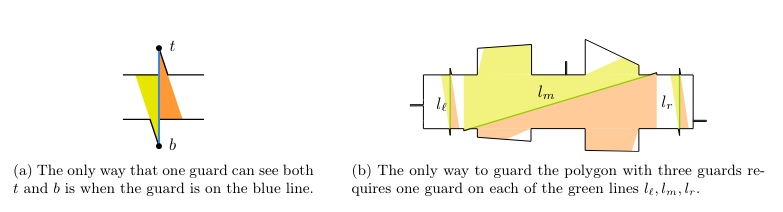
\includegraphics[width=\textwidth]{Screenshot from 2022-02-02 09-57-44.png}
    \caption{Forcing Guards to Lie on Specific Line Segments.}
    \label{fig:tb}
\end{figure}

\subsubsection{Intuition for Quadrilaterial Pockets}
The four quadrilateral pockets are created in order to force a guard in a region bounded by a curve. Figure \ref{fig:quadrilateral_pockets} depicts the visualisation for this case. Considering the fixed position of a guard $g_m$ either on the left or on the right of the curve $c_\ell$, there exists a position of guard $g_\ell$ on $l_\ell$ such that edge $e_t^\ell$ and line $p_b^{\ell}g_m$ are seen by $g_\ell$. Then, only if $g_m$ is on the left or on $c_\ell$ can it see the remaining parts of the pockets that are not seen by $g_\ell$ (edge $e_b^{\ell}$, line $p_t^{\ell}g_{\ell}$). Analogously, in order for the right side of $\mathcal P$ and the right pair of quadrilateral pockets to be seen by both guards $g_m$ and $g_r$, $g_m$ has to be on the curve $c_r$ or on its right. Since $g_m$ has to also satisfy its position on $c_\ell$, its only feasible position is as the intersection point between $c_\ell$ and $c_r$. 

\begin{figure}[h!]
    \centering
    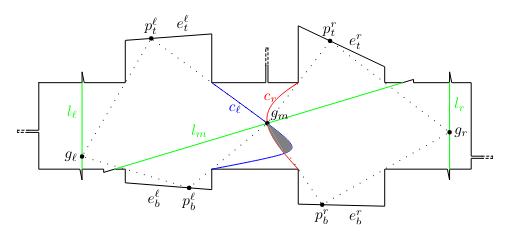
\includegraphics[width=0.7\textwidth]{Screenshot from 2022-01-21 12-02-44.png}
    \caption{Restricting a Guard to a Region Bounded by a Curve}
    \label{fig:quadrilateral_pockets}
\end{figure}

\subsubsection{Intuition for Rectangular Pockets}
The three rectangular pockets are created in order to force a guard to a single irrational point. Further building onto the previously discussed instance from Figure \ref{fig:quadrilateral_pockets}, the three rectangular pockets on the laterals and top of $\mathcal P$ are added.  They then allow for additional constraints for the positions of the guards $g_\ell, g_m, g_r$. Based on the curve equations of $c_\ell$ and $c_r$, we can thus calculate the irrational position of $g_m = (3.5 + 5\sqrt 2, 1.5\sqrt 2)$. Subsequently, we can fix the positions of $g_\ell$ and $g_r$ on lines $l_\ell$ and $l_r$.

\subsubsection{Monotone Polygon Creation}
The polygon $\mathcal P$ in question  was then found through experimentation in GeoGebra\footnote{\url{https://www.geogebra.org/}}. The triangular and rectangular pockets were fixed. Finding then the position of the rectangular pockets required the existence of a rational line that contained the irrational coordinates of guard $g_m$ from Figure \ref{fig:quadrilateral_pockets}. The irrational coordinates of the two other guards $g_\ell, g_r$ were chosen such that they would be able to see the rest of the polygon that is unseen by $g_m$. The rectangular pockets were added based on their coordinates.

In this way, dependencies between guard positions were created with each guard placed on each of the lines $l_\ell, l_m, l_r$ at unique irrational positions. The guard set becomes thus $S = \{g_\ell, g_m, g_r\}$.  Given the properties of the positions of the guards (unique and irrational), the only method to seeing the whole polygon $\mathcal P$ using guards with rational positions would be to use more than 3 (at least 4). This statement can also be generalised such that a family of polygons $(\mathcal{P}_n)_{n \in \mathbb{Z}_+}, \forall n$ can be guarded by $3n$ guards with irrational coordinates, or $4n$ guards with rational coordinates. The coordinates determining the polygons are hence polynomial in $n$.

\subsubsection{Rectilinear Polygon Creation}
Similarly, a rectilinear polygon $\mathcal P_R$ can be created given integer coordinates. $\mathcal P_R$ would require guards with irrational coordinates in any optimal solution. It can be guarded by 9 guards if guards can be placed at points with irrational coordinates. Otherwise, the smallest optimal guard set $S$ with rational coordinates would be of size 10.

$\mathcal P_R$ can be thus constructed by extending $\mathcal P$ with the 6 non-rectiliniar gray parts ($Q_1, Q_2, Q_3, Q_4, T_1, T_2$) in Figure \ref{fig:rectilinear}, such that each of them requires at least 1 guard in the interior. When placing 6 guards in the gray parts, the white areas of $\mathcal P_R$ remain unseen. As such, 3 guards must still be similarly placed at the 3 irrational points on lines $l_\ell, l_m, l_r$ as in the case of $\mathcal P$, in order to guard the rest of $\mathcal P_R$.

\begin{figure}[h!]
    \centering
    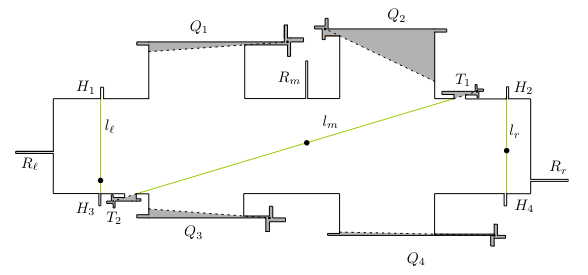
\includegraphics[width=0.7\textwidth]{Screenshot from 2022-01-21 12-46-51.png}
    \caption{Rectilinear Polygon $\mathcal P_R$}
    \label{fig:rectilinear}
\end{figure}
% a guard at position $x$ sees a point $y$ if the line segment $xy$ is fully contained in the polygon $\mathcal{P}$
% - a _guard set_ $S$ is a set of points in $\mathcal{P}$ s.t. every point in $\mathcal{P}$ is seen by some point in $S$ - find a minimum cardinality guard set for a simple polygon $\mathcal{P}$ on $n$ vertices
% - research less focussed on the classical problem, but more on its variations
% - no combinatorial algorithm for finding an optimal solution, or even for deciding whether a guard set of a given size $k$ exists, only real algebraic geometry powerful tools - not known if in NP
% - given polygons by integer coordinates, do they require guard positions with irrational coordinates in any optimal solution?
	% => yes, by constructing a _monotone_ polygon ($\exists$ line $l$ s.t. every line orthogonal to $l$ intersects $\mathcal P$ at most twice) with integer coordinates that can be guarded by three guards only when we allow to place the guards at points with irrational coordinates; otherwise, 4 guards are needed
			% - *place pic*
			% - **forcing a guard on a line segment** by creating 3 triangular pockets *pic* that can enforce 3 guards on 3 line segments within $\mathcal P$ - a guard can see both $t$ and $b$ if it is on the blue line segment $tb$, which is the intersection of 2 regions => $k$ pairs of triangular pockets and no 2 regions corresponding to different pairs of pockets intersecting => in order to guard the polygon with $k$ guards, there must be one guard on the line segment corresponding to each pair
			% - **restricting a guard to a region bounded by a curve** - consider a fixed position of $g_2$ on or to the right of the segment $bd$. $\exists$ a position of $g_1$ on $l$ s.t. the entire polygon is seen by $g_1$ and $g_2$ iff. $g_2$ lies on or to the left of the curve $\mathcal C$ *insert pic*
			% - **restricting a guard to a single (irrational) point** - *insert pic* $g_m$ and $g_l$ can guard together the 2 left pockets, and at the same time $g_m$ and $g_r$ can guard together the two right pockets => $g_m$ can only be in the irrational point $p = (3.5 + 5\sqrt 2, 1.5\sqrt 2)$
			% - **searching for the polygon** - we need to force $g_m$ to be on a line $l_m$ containing $p$, but we can only force $g_m$ to be on a rational line => we require the existence of a rational line $l_m$ that contains $p$ - there can be at most one rational line containing the irrational point $p$, as any 2 rational lines intersect in a rational point => reverse-engineer the polygon, after having chosen the positions of the guards of the form $(r_1 + r_2\sqrt 2, r_3 + r_4\sqrt 2), r_1, r_2, r_3, r_4 \in \mathbb Q$ ; rectangle with pockets added
	% - consider any set $S$ for $\mathcal P$ consisting of at most 3 guards: then $|S| = 3$ and $\exists$ 1 guard on each of the lines $l_l, l_m, l_r$
	% - consider any guard set $S$ for $\mathcal P$ consisting of 3 guards; then 1 of the guards has an $x$-coord in $[10.5, 10.6]$. For the remaining 2 guards, $g_l$ has a $y$-coord in $i_1 = [0.5, 0.6]$ and the $g_r$ in $i_2 = [1.7, 1.8]$
	% - **dependencies between guard positions**
		% - the guards $g_l$ and $g_m$ together see all of $e_t^l$ and $e_b^l$ and the guards $g_m$ and $g_r$ together can see all of $e_t^r$ and $e_b^r$ *add pic*
	% - **computing the unique solution**
		% - the max $x$-coord of $g_m$ s.t. $g_l$ and $g_m$ can together see $e_t^l$ and $e_b^l$ is $x = 3.5 + 5\sqrt 2$. The corresponding position of $g_l$ is $(2, 2 - \sqrt 2)$
		% - the min $x$-coord of $g_m$ s.t. $g_r$ and $g_m$ can see both $e_t^r$ and $e_b^r$ is $x = 3.5 + 5\sqrt 2$. The corresponding position of $g_r$ is $(19, 1 + \frac{\sqrt 2}{2})$  
	% - $\forall n$, there is a family of polygons $(\mathcal{P}_n)_{n \in \mathbb{Z}_+}$ which can be guarded by $3n$ guards with irrational coordinates, but need $4n$ guards to be rational; the coordinates of the points defining the polygons $\mathcal P_n$ are polynomial in $n$
	% - there is a rectilinear polygon $\mathcal P_R$ given by integer coordinates that require guards with irrational coordinates in any optimal solution - $\mathcal P_R$ can be guarded by 9 guards if we allow placing guards at points with irrational coordinates; an optimal guard set of $\mathcal P_R$ with guards at points with rational coordinates has size 10
		% - start with $\mathcal P$ - extend the non-rectilinear parts by "equivalent" rectilinear parts (gray) s.t. each of them requires at least  1 guard in the interior; if the interior of each pocket contains only 1 guard, then these guards must be placed at specific positions, making the area not seen by these 6 additional guards (white) => the remaining 3 guards must be placed at 3 irrational points (*place pic*)
% - _terrain guarding problem_ - $x$-monotone polygonal curve $c$ is given, the region $R$ above $c$ has to be guarded, and the guards are restricted to lie on $c$ - discretisation available in $O(n^3)$ time -> no irrational numbers phenomenon, and the decision version of the terrain guarding problem is in NP
\newpage
\subsection{Implementation of Polygon Guarding Algorithms for Art Gallery Problems \cite{maleki2022implementation}}
Maleki abd Mohades \cite{maleki2022implementation} introduce the implementations and their experimental evaluations for two existing approximation algorithms (\cite{GHOSH2010718}, \cite{bhattacharya2016approximability}) and a newly developed one for computing visibility in simple polygons in the context of the Art Gallery Problem \cite{o1987art}.

We distinguish between vertex guards (guards that can be placed on the vertices of $\mathcal P$) and point guards (guards that can be placed without restriction inside $\mathcal P$). If $\forall q \in \mathcal P$ is visible from some point of an edge, then $\mathcal P$ is a weak visibility polygon.

Given that computing a minimum number of guards for guarding a polygon is NP-hard \cite{1057165}, Maleki and Mohades will inspect how the Art Gallery Problem \cite{o1987art} can be tackled using three approximation algorithms.

\subsubsection{Algorithm of Ghosh \cite{GHOSH2010718}}
The algorithm of Ghosh \cite{GHOSH2010718} runs in $O(n^4)$ time and yields a $O(\log n)$-approximation for computing the minimum vertex guard for simple polygons. It begins by drawing lines through every pair of vertices of $\mathcal P$ and computing the set of all its convex components $C$. It continues by adding the elements of $C$ that are visible from vertex $j, \forall j$ into the set $F_j$. Then, it recursively eliminates the redundant sets $F_i$ from $C$ as follows: $\forall$ fixed $j$, another vertex $i$ is searched for such that the set $F_i$ is also visible from $j$ ($|F_j| \leq |F_i|$); $F_i$ is eliminated from $C$, $i$ is added to $S$ and the process continues until $C$ is empty. At the end, $S$ contains the approximated guardset for $\mathcal P$.

\subsubsection{Algorithm of Bhattacharya \cite{bhattacharya2016approximability}}
The algorithm of Bhattacharya \cite{bhattacharya2016approximability} runs in $O(n^2)$ time and yields a 6-approximation for computing the minimum vertex guard for weak visibility polygons without holes. It begins by choosing two neighbours $u, v$ as parents for every vertex in $\mathcal P$. It then computes the Shortest Path Tree from each pair of parents $u, v$ to every other vertex in $\mathcal P$. All vertices on the Shortest Path Tree are initialised as unmarked. In clockwise order from $\overline{uv}$, every vertex $z \in \mathcal P$ is checked for visibility from $u, \text{ and } v$. If all vertices $z$ are visible, then $u, \text{ and }v$ are added to $S$. Otherwise, $z$ is added to $S$ and the procedure continues with $z$ as the starting node. All vertices that become seen from $S$ are marked. At the end, the algorithm checks whether the vertices in $S$ have overlapping visibility regions, and duplicates are removed.

\subsubsection{New Algorithm}
The algorithm introduced by Maleki and Mohades is focussed on polygons with large number of vertices $n$ and different amounts of reflex vertices $r$. If the number of reflex vertices is significantly lower than the total number of vertices ($r \leq \log \log n$), guards are placed at all reflex vertices. Otherwise, they are placed according to the algorithm of Ghosh \cite{GHOSH2010718}.

\subsubsection{Experiments}
Algorithms of Ghosh \cite{GHOSH2010718} and Bhattacharya \cite{bhattacharya2016approximability} are tested on weak visibility polygons, and the newly introduced algorithm is tested on simple polygons. 

Firstly, a procedure for generating arbitrary weak visibility polygons is devised in Figure \ref{fig:weak}: given two points $p = (k, 0), q = (-k, 0)$,  $n$ random points $\{x_1, ..., x_n\}$ sorted on the distance from $p$ on $\overline{pq}$, $n$ sorted random angles $\{\alpha_1, ..., \alpha_n\} \in  (0, \pi)$, and $n$ vertices $\{y_1, ..., y_n\}$ are created by shooting $n$ rays at the corresponding angle $\alpha_i, \forall x_i$. Then, $n$ reflex vertices $\{z_1, ..., z_n\}$ are added in the quadrilateral formed by vertices $x_iy_iy_{i + 1}x_{i + 1}$. The figure is accredited to \cite{maleki2022implementation}.

\begin{figure}[h!]
    \centering
    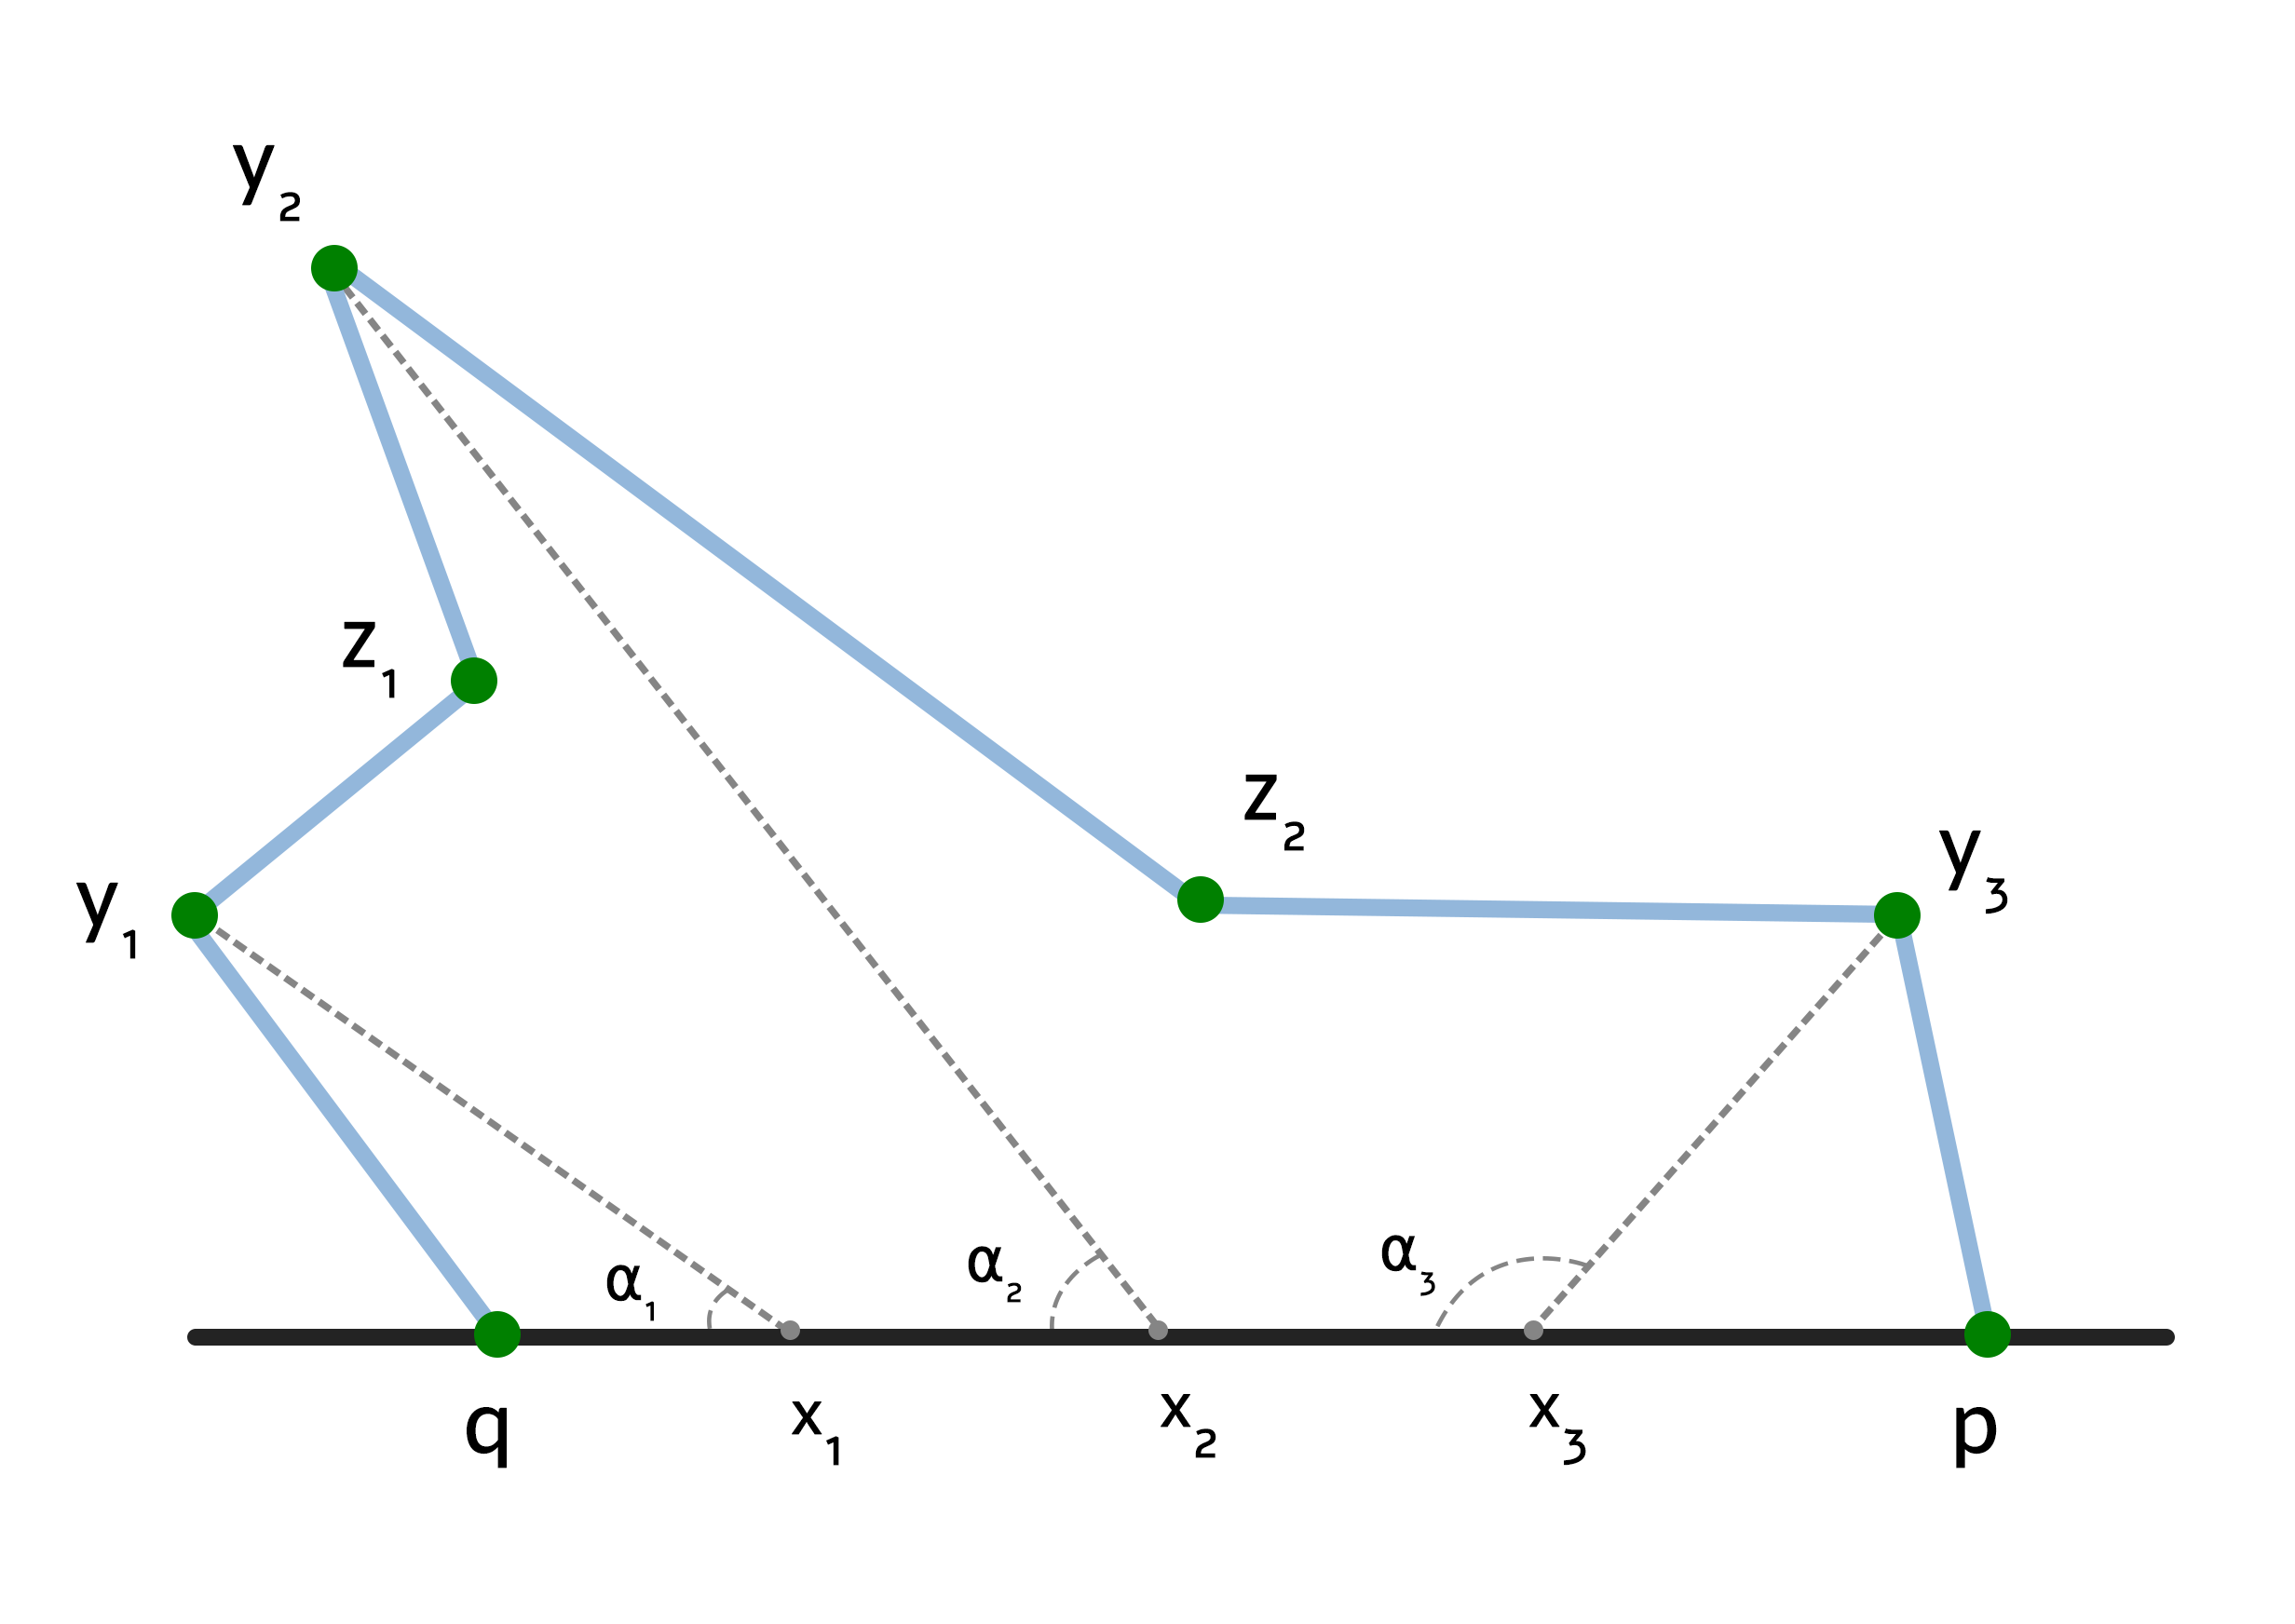
\includegraphics[width=0.6\textwidth]{weak.png}
    \caption{Generated Weak Visibility Polygon for $n = 3$ \cite{maleki2022implementation}.}
    \label{fig:weak}
\end{figure}

The algorithms of Ghosh \cite{GHOSH2010718} and Bhattacharya \cite{bhattacharya2016approximability} were tested using arbitrarily generated polygons with $n = \overline{10, 15}$ vertices and $r \in \{2, 3\}$ reflex vertices. The results suggest that for low values of $n$ and $r$, the algorithm of Ghosh \cite{GHOSH2010718} performs better when using the number of guards as evaluation criteria. 
% Its constant time approximation in the small case contrasts with the constant approximation of the algorithm of Bhattacharya \cite{bhattacharya2016approximability}.
Similarly, the algorithm of Ghosh \cite{GHOSH2010718} performed better both when tested on a weak visibility polygon with low $n = \overline{10, 15}$ and $\frac n 2 \leq r$, and when tested with large $n \in \{100, 400\}$.

Secondly, a procedure for generating arbitrary simple polygons with custom number of reflex vertices $r$ is devised in Figure \ref{fig:arbitrary}. The figure was taken from \cite{maleki2022implementation} and annotated to suit the explanations in these summaries. Starting from a simple convex polygon $\mathcal P$ with $n$ vertices ($u, v, x1, x2, ..., x7$), $\mathcal P$ is triangulated such that every triangle has a joint edge with its boundaries; $r$ reflex vertices ($r1, r2, r3$) are randomly added inside $\mathcal P$, and the boundaries outside of the reflex vertices are moved such that all $r$ points are now forming boundaries. 

\begin{figure}[h!]
    \centering
    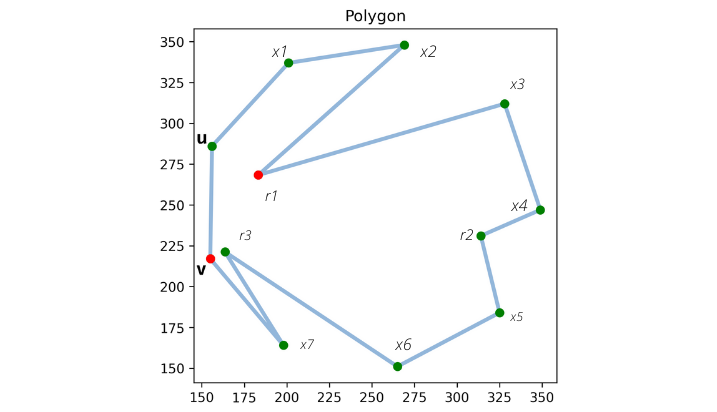
\includegraphics[width=0.7\textwidth]{concave_test.png}
    \caption{Generated Arbitrary Simple Polygon $\mathcal P$ for $n = 12, r = 3$ \cite{maleki2022implementation}.}
    \label{fig:arbitrary}
\end{figure}

The new algorithm is tested on simple polygons constructed as mentioned by starting from low $r$ and gradually increasing it. The results are reported positively in the sense that the $|S|$ always remains close to the optimal, as a 2-approximation solution.

Therefore, through the newly implemented algorithm, Maleki and Mohades \cite{maleki2022implementation} testify that the algorithm of Ghosh \cite{GHOSH2010718} performs like a constant approximation in practice, and often better than its theoretical bound when tested on complex simple polygons.
% - guards placed on vertices = vertex guards
% - no restrictions = point guards
% - $\mathcal P$ is called weak visibility polygon if every point in $\mathcal P$ is visible from some point of an edge
% - the problem of computing a min number of guards is NP-hard
% - $O(n^4)$ approximation algorithm for computing $S$ (1)
% - $O(n^2)$ 6-approximation algorithm for vertex \subsection{Implementation of Polygon Guarding Algorithms for Art Gallery Problems \cite{maleki2022implementation}}
% - guards placed on vertices = vertex guards
% - no restrictions = point guards
% - $\mathcal P$ is called weak visibility polygon if every point in $\mathcal P$ is visible from some point of an edge
% - the problem of computing a min number of guards is NP-hard
% - $O(n^4)$ approximation algorithm for computing $S$ (1)
% - $O(n^2)$ 6-approximation algorithm for vertex guarding a weak vibisility $\mathcal P$ with no holes (2)
% - implementation of algorithms and testing on weak visibility polygons
% - generating arbitrary weak visibility polygons *add algorithm* and testing them with $n = \overline{10, 15}$ and $r \in \{2, 3\}$ reflex vertices
	% - for low value of $n$ and $r$, it is better to use Algorithm 1 for minimising the number of vertex guards; since algorithm 2 is a constant approximation algorithm, algorithm 1 performs like a constant time approximation algorithm for small values of $n$ and $r$ experimentally
	% - since the criteria of minimisation is the number of guards rather than the running time which is a one-time affair unlike online algorithms, algorithm 1 is preferable even for weak visibility polygons
% - generating arbitrary weak visibility polygons and testing them with $n = \overline{10, 15}$ and $r$ reflex vertices close to the number of convex vertices
	% - for a low value of $n$ and $\frac n 2 \leq r$, algorithm 1 is better for guarding a weak visibility polygon with a min number of guards, because when the number of reflex vertices increases, the number of the diameter of the polygon and convex components decrease
% - generating arbitrary weak visibility polygons and testing them with large $n$
	% - algorithm 1 is better for guarding a weak visibility polygon with min number of guards, because it uses less guards than algorithm 2
% - generating arbitrary simply polygons *add algorithm* (Ghosh)
% - if $r << n$ , then the size of the optimal guard set is $\approx r$  => the number of edges $E$ in the visibility graph of such simple polygons is $O(n^2)$ => choose a small number $\log \log n$ as an upper bound for $r$ so that $r$ and optimal are close
% - if $r - c \leq \log \log n$, $c$ - small constant, then we place guards at all reflex vertices for guarding a simple polygon $P$, otherwise we place guards using the method of algorithm 1
% - even if $E$ reduces, the chosen guard sets remains close to the optimal and the algorithm assigns no more than twice the optimal number of guards
% => Ghosh's idea works better in practice and performs like a constant approximation algorithmalgorithm 2 is a constant approximation algorithm, algorithm 1 performs like a constant time approximation algorithm for small values of $n$ and $r$ experimentally
	% - since the criteria of minimisation is the number of guards rather than the running time which is a one-time affair unlike online algorithms, algorithm 1 is preferable even for weak visibility polygons
% - generating arbitrary weak visibility polygons and testing them with $n = \overline{10, 15}$ and $r$ reflex vertices close to the number of convex vertices
	% - for a low value of $n$ and $\frac n 2 \leq r$, algorithm 1 is better for guarding a weak visibility polygon with a min number of guards, because when the number of reflex vertices increases, the number of the diameter of the polygon and convex components decrease
% - generating arbitrary weak visibility polygons and testing them with large $n$
	% - algorithm 1 is better for guarding a weak visibility polygon with min number of guards, because it uses less guards than algorithm 2
% - generating arbitrary simply polygons *add algorithm* (Ghosh)
% - if $r << n$ , then the size of the optimal guard set is $\approx r$  => the number of edges $E$ in the visibility graph of such simple polygons is $O(n^2)$ => choose a small number $\log \log n$ as an upper bound for $r$ so that $r$ and optimal are close
% - if $r - c \leq \log \log n$, $c$ - small constant, then we place guards at all reflex vertices for guarding a simple polygon $P$, otherwise we place guards using the method of algorithm 1
% - even if $E$ reduces, the chosen guard sets remains close to the optimal and the algorithm assigns no more than twice the optimal number of guards
% => Ghosh's idea works better in practice and performs like a constant approximation algorithm
\subsection{A Practical Algorithm with Performance Guarantees for the Art Gallery Problem \cite{DBLP:journals/corr/abs-2007-06920}}
Hengeveld and Miltzow \cite{DBLP:journals/corr/abs-2007-06920} introduce the idea of vision-stability, and describe an iterative algorithm that guarantees to find the optimal guard set for every vision-stable polygon in order to address the Art Gallery Problem \cite{o1987art}. Additionally, it proves that the set of vision-stable polygons admits an FPT algorithm when parametrised by the number of vertices visible from a chord of the polygon, and gives a one-shot algorithm for that matter.

Hengeveld and Miltzow \cite{DBLP:journals/corr/abs-2007-06920} start by introducing the notion of vision-stability in Figure \ref{fig:vis}. The figure was taken from \cite{DBLP:journals/corr/abs-2007-06920} and annotated to facilitate the understanding of this summary. The authors define guards as ``enhanced'' if they can ``see around the corner'' by an angle of $\delta$ ($vis_\delta(p)$), or ``diminished'' if their vision is ``blocked'' by reflex vertices by an angle of $\delta$ ($vis_{-\delta}(p)$). As such, the size of the minimum $\delta$-guarding set is defined as $opt(P, \delta)$. A polygon $\mathcal P$ has vision-stability $\delta$ if the optimal number of enhanced guards is the same as the optimal number of diminished guards for that matter ($opt(P, -\delta) = opt(P, \delta)$). 

\begin{figure}[h!]
    \centering
    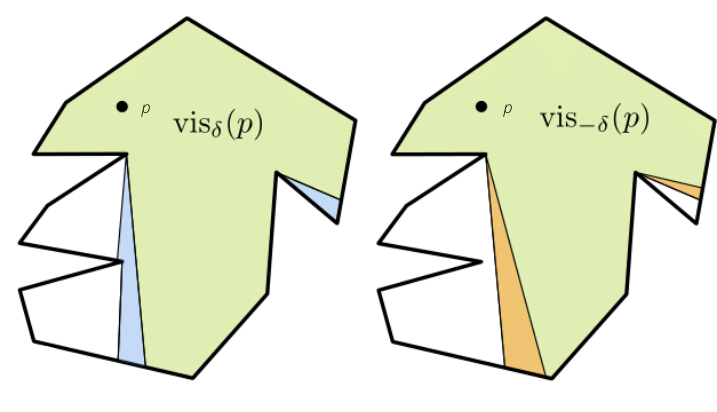
\includegraphics[width=0.5\textwidth]{vis_delta.png}
    \caption{Enhanced ($vis_\delta(p)$) and Diminished ($vis_{-\delta}(p)$) Visibility Regions of $p$ \cite{DBLP:journals/corr/abs-2007-06920}.}
    \label{fig:vis}
\end{figure}

Let $C$ be the candidate guard set and $W$ the witness guard set that will be later used in the algorithm. Firstly, rays are shot from every reflex vertex such that the angle between any two rays is at most $\delta$, as observed in Figure \ref{fig:rays}, as taken from \cite{DBLP:journals/corr/abs-2007-06920}. All the intersection points of the rays within $\mathcal P$ define the candidate guard set $C$, together with the faces they are part of. A witness guard set $W$ is then defined by picking an arbitrary interior point of every face of $\mathcal P$, together with all faces of $\mathcal P$. In this way, the problem can be discretised in a way in which the solution to the discretised problem are also solutions to the continuous problem.

\begin{figure}[h!]
    \centering
    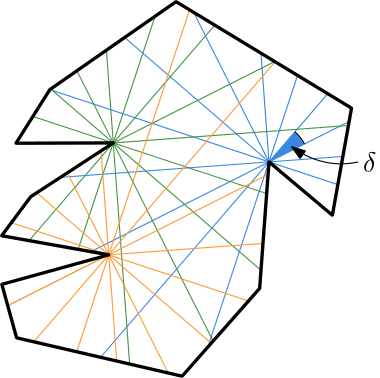
\includegraphics[width=0.3\textwidth]{Shooting-1.png}
    \caption{Shooting Rays from All Reflex Vertices with Angles between Them at Most $\delta$ \cite{DBLP:journals/corr/abs-2007-06920}.}
    \label{fig:rays}
\end{figure}


\subsubsection{One-Shot Vision-Stable Algorithm}
At first, an Integer Program (IP) is built and named the One-Shot Vision-Stable Algorithm. It computes the minimum number of point guards in polynomial time in a vision-stable polygon $\mathcal P$ with  vision-stability $\delta$ and $r$ reflex vertices. The guards are encoded by binary integers, and linear equations and inequalities are used to encode visibility. Assuming that $\delta$ is part of the input, the algorithm returns the optimal solution only if the vision-stability of $\mathcal P$ is larger or equal to $\delta$. The one-shot vision-stable algorithm is reliable, as it also verifies that its result is an optimal solution. It is also FPT with respect to $r$. As such, the optimisation function $f_1$ of the IP is $$f_1 = (\sum_{c \in vertex(C)} c) + ((1 + \epsilon)\sum_{c \in face(C)} c) + (\epsilon \sum_{w \in face(W)} w), \frac 1 \epsilon = |C| + |W| + 1.$$ For every witness $w$, its visible set of candidates are denoted as $vis(w)$, where $face$ and $vertex$ refer to whether the candidate is a face or a vertex, respectively.

Additionally, a constraint for each vertex and face witness $w$ to be respectively seen by all candidates from $vis(w)$ is added:
% \begin{equation}
	\begin{align*}
		\sum_{c \in vis(w)} c &\geq 1, \forall w \in vertex(W) \\
		w + \sum_{c \in vis(w)} c &\geq 1, \forall w \in face(W).
	\end{align*}
% \end{equation}

Nonetheless, the one-shot vision-stable algorithm proves to be too slow for practical reasons. The bottleneck is however not solving the IP in itself, but computing visibilities. Hence, an iterative vision-stable algorithm is devised, that is faster and retains similar performance guarantees. 

\subsubsection{Iterative Vision-Stable Algorithm}
Starting with the same sets of candidates $C$ and witnesses $W$, another IP is deployed in order to find a minimum guard set $S \subseteq C$ that sees all vertex-witnesses. This algorithm is then called the Iterative Vision Stable Algorithm, as it makes use of both the One-Shot IP and the new one. 

At first, the new IP builds on the One-Shot IP by forming $W^* \subseteq W$ as a critical witnesses set with only 10\% randomly selected vertices from $W$. $W^*$ is expanded throughout the iterations with the witnesses that are not seen by the optimal solution at that moment. The new IP is referred to as the Big IP.
Then, the Big IP receives a secondary objective function $f_2$ (Equation \ref{eq:f2}). $f_2$ minimises the number of face-guards used in $S$ and the number of unseen face-witnesses. If $S$ contains only point guards and sees all face-witnesses, the algorithm reports the optimal solution by using the One-Shot IP. Otherwise, the faces of $\mathcal P$ are split (discretised) and the algorithm continues to the next iteration. The One-Shot IP is then used as soon as all faces are deemed unsplittable (they have reached a certain granularity $\lambda$). In that case, the Big IP is run again. The Big IP consists thus of a similar objective and constraints as the One-Shot Vision-Stable IP: besides assuring that all witnesses $w$ are seen by their set of candidates $vis(w)$, it also enforces that only the number of guards $s$ resulted from the One-Shot IP is used, as follows: 
\begin{align}
	f_2 &= \sum_{x \in splittable(W \cup C)} x \label{eq:f2}\\
	\sum_{c \in C} c &= s, s \in \mathbb Z, s \text{ the number of used guards in the One-Shot IP} \\
	\sum_{c \in vis(w)} c &\geq 1 \\
	1 - (\epsilon \sum_{c \in vis(w)} c) &\geq w.
\end{align}

The Iterative Algorithm is then transformed into an FPT algorithm with the parameter of chord-visibility width. Given a chord $c$ of $\mathcal P$, we count the number $n(c)$ of vertices visible from $c$. The chord-visibility width of $\mathcal P$ ($cw(P)$)  is the maximum $n(c)$ over all possible chords $c$. By using this measure, it is possible to describe the local complexity of a polygon: many synthetic arbitrary polygons have much smaller chord-visibility width than they have reflex vertices, and polygons constructed with hardness reductions have the chord-visibility width proportional to the total number of vertices. 

\subsubsection{Experimental Results}
The previously introduced algorithms are tested experimentally in terms of their running times and solution quality with respect to the input size, chord-visibility width and vision-stability of the input polygons $\mathcal P$. The tests were run on 30 instances of arbitrary simple polygons of sizes 60, 100, 200 and 500 vertices. The algorithms have been implemented both with the theoretical performance guarantees $\mathcal T$ (if no solution is found in $\mathcal T$, abort) and with the practical optimisation of critical witnesses.

When running the Iterative Algorithm with optimisations, reasonable practical results were found: all tested instances were solved to optimality, although the overall running time was not improved when compared to state-of-the-art algorithms. The median running time was also lower than the average running time, which could be accounted for by the sensitivity of the algorithm to the vision-stability of a polygon. Thus, a few polygons that are hard to solve (have low vision-stability) outweigh the rest of the running times.

When running the iterative algorithm without optimisations and with the theoretical limit $\mathcal T$ as a safe guard, a solution was found in an efficient manner (within an hour) only for 25 out of 30 instances. For the rest of the 5 instances, the Big IP performed unnecessary splits, which negatively influenced the running times.

Additionally, the correlation between the granularity $\lambda$ of the input polygon was tested for the iterative algorithm with performance guarantees $\mathcal T$. There appeared to be a strong correlation between the running times and $\lambda$. Thus, lower granularity implied a shorter running time.

In terms of the convergence to the optimal solution, the iterative algorithm with optimisations has been used to show the fast convergence in the first few iterations. The speed of the convergence slows down as the algorithm nears its end due to the increasing number of candidates and witnesses that are added to $C$ and $W^*$, respectively, in the later iterations. Nonetheless, it appears that computing the visibility area of the polygon is still the bottleneck in the algorithm's performance.



% _practice-theory gap_; $\exists \mathbb{R}$-complete
% - encode guards by real numbers and use polynomial equations and inequalities to encode visibility
% - optimal solutions found on synthetic instances of up to 5k vertices => discretise the problem and hope that the discretised problem also gives the optimal solution to the original problem
	% - generate a _candidate_ set $C$ and a _witness_ set $W$, compute the optimal way to guard $W$ using the min number of guards in $C$
	% - more candidates and witnesses are generated until the optimal solution is found
	% - find a min guard set $G \subseteq C$ that sees all vertex-witnesses
	% - secondary objective function: minimise the number of face-guards used in $G$ and the number of unseen face-witnesses
	% - if $G$ contains only point guards and sees all face-witnesses => optimal solution; otherwise it refines $\mathbb{A}$ and goes to the next iteration
% - given a closed simply polygon $P$ we say 2 points $p, q$ see each other if the segment $seg(p, q)$ is fully contained in $P$
% - the art gallery problem seeks a min size set $G \subset P$ of guards that sees $P$ completely
% - notion of _vision-stability_
	% - consider an _enhanced_ guard that can see "around the corner" by an angle of $\delta$ or a _diminished_ guard whose vision is by an angle of $\delta$ "blocked" by reflex vertices
	% - a polygon $P$ has vision-stability $\delta$ if the optimal number of enhanced guards to guard $P$ is the same as the optimal number of diminished guards to guard $P$
	% - shoot rays from every reflex vertex, s.t. the angle between any 2 rays is at most some given angle $\delta$; all intersection points of the rays within the polygon $P$ define our candidate set $C$
	% - $vis_\delta(p)$ - enhanced visibility
	% - $vis_{-\delta}(p)$ - diminished visibility regions of points
	% - $opt(P, \delta)$ - size of the min $\delta$-guarding set
	% - $opt(P, -\delta) = opt(P, \delta)$ - vision-stability
	% - _visibility-enhancing region_ $A = A(q, r, \delta)$
	% - don't know how to test it for a specific value $\delta$
% - _one-shot vision-stable_ algorithm that computes an optimal guard set for vision-stable polygons using polynomial time and solving one IP - finds the optimal solution for every vision-stable polygon
	% - the bottleneck is not solving the IP, ol
		% 	- normal protocol - square splits only if the face is incident to more than one reflex vertex; choose angular split with probability 0.8, and the other two remaining split types with equal probabilities; in case a split is impossible, we will try the two other splits, before deciding that a face is unsplittable
		% 	- square spthms
	% - the art gallery problem is in NP for vision-stable polygons
	% - _reliable_ - even if the input polygon is not vision-stable, the reported result is correct
	% - refine by splitting appropriate faces
	% - work with _critical witnesses_
	% 	- initialise the critical witness set $W^*$ by randomly picking 10\% of vertices and faces, for each weak visibility polygon
	% 	- compute all the vertices and faces that the IP $G$ sees (the sets of unseen face-witnesses and vertex-witnesses), then randomly choose a small constant size subset of vertices and faces from $U$ that we add to $W^*$ - find a good balance between adding too few critical witnesses and too many
	% 	- every time we update the critical witness set, rerun the IP to check if we can find a better solution given the critical witnesses; we keep adding to the critical witness set as long as there are unseen witnesses left that are not marked as critical; check if we need to update the new critical witness set again using the new-found guard set (critical cycles); repeat until we find a guard set that can see the entire polygon -> split the faces and continue with the next iteration
	% 	- we do not need to compute all the visibilities between all the candidates and all witnesses; compute all visibilities between the critical witnesses $W^*$ and candidates $C$ and then all visibilities between the guards $G$ and the witnesses $W$
	% 	- _delayed critical witness protocol_ - use critical witnesses and add all faces, which have a power larger than the granularity $\sqrt \lambda$ 
	% - _weak visibility polygon tree_ - exploit low local complexity in order to reduce the number of visibility queries to be answered
		% - start with an arbitrary edge $e$ on the boundary of $P$ -> compute the weak visibility polygon $vis(e)$ of $e$ which is the root of $T$: $\forall e'$ of $vis(e)$ which is not part of the boundary of $P$, we compute the weak visibility polygon $vis(e')$ w.r.t. the polygon $P - vis(e)$ => children of $vis(e)$
		% - $\forall$ node of $T$ is a weak visibility polygon $W$ of some defining chord $c$ => $c$ splits $P$ into 2 polygons $Q$ and $Q'$; the weak visibility polygon $W$ is completely contained in either $Q$ or $Q'$ (consider each node of $T$) to be closed and contain its boundary
		% - initialisation: construct an arrangement $A$, where we add defining chords $c$ of the weak visibility polygon tree to $A$, shot horizontal and vertical rays from each reflex vertex, stop as soon as it hits the boundary or another edge of $A$
		% - splits:
		% 	- square splits - divide a face using a horizontal and vertical segment, s.t. the height and the width of the new faces are halved
		% 	- angular splits - shoot rays from a reflex vertex as to reduce the power of the face
		% 	- reflex chord splits - do them if no other type of split is possible
		% 	- extension splits - given a reflex vertex $r$, we can consider the rays with apex $r$ parallel to the two incident edges of $r$
		% 	- unsplittable faces - the face is incident to at most one reflex vertex + no reflex chord or extension split is possible + the face is not splittable by angular splits of granularity $\lambda$ 
		% - protocol
		% 	- normal protocol - square splits only if the face is incident to more than one reflex vertex; choose angular split with probability 0.8, and the other two remaining split types with equal probabilities; in case a split is impossible, we will try the two other splits, before deciding that a face is unsplittable
		% 	- square split protocol - always use square splits
% - building the IP
	% - normal IP - one-shot IP, only adds constraints and variables for critical witnesses
		% - if $G$ contains only vertex-guards and we checked that $G$ sees the entire polygon, then the algorithm reports $G$ as the optimal solution; else continue with the next iteration; else use the big IP
	% - big IP - find a solution with at least one unsplittable face, maximise the number of splittable faces that are used
% - granularity update protocol - replace $\lambda$ by $\frac \lambda 2$ (_normal granularity update protocol_), or by $\lambda^2$ (_accelerated granularity update protocol_) - use almost exclusively the simple IP protocol; accelerated seems to combine the best of both worls
% - given a chord $c$ of a polygon, $n(c)$ number of vertices visible from $c$
	% - _chord-visibility width_ $cw(P)$ of a polygon is the max $n(c)$ over all possible chords $c$
	% - the set of vision-stable polygons admit an FPT algorithm, when parametrised by the chord-visibility width

% - run practical algorithm $\mathbf{P}$ within the running time bound of $\mathbf{T}$(safe-guard), abort if no solution 
% - test the algorithm on several input polygons (30 instances of sizes 60, 100, 200 and 500 vertices) with algorithm that has theoretical performance guarantees and optimised one
% 	- iterative algorithm without safe guards - used critical witness protocol with normal split protocol and simple IP - find optimal solutions for all tested instances, performs similar to other algorithms, but susceptible to the vision-stability of the algorithm
% 	- iterative algorithm with safe guards - no critical witnesses, normal split protocol, normal IP protocol
% 		- efficient solution for 25/30 instances for 60-vertices polygon
% 	- correlation of granularity and running time - min granularity $\lambda$ might not be the best indication of the vision-stability of a polygon (discretisation); random IP splits choice, chord-visibility width influence
% 	- distribution of CPU usage - the running time of the algorithm is dominated by the face-visibility queries combined with the weak visibility decomposition